Curvas elípticas se definem por equações cúbicas com grau 3, um exemplo é a equação: $y^2 = x^3 - x$. Na figura \ref{fig:curvas} é possível observar a curva mencionada anteriormente e a $y^2 = x^3 -x + 1$ para exemplificar o formato de uma curva elíptica. Umas das funcionalidades das curvas é provar o último teorema de Fermat que diz que uma equação $x^n + y^n = z^n$, quando $n > 2$, não possui uma solução com inteiros diferentes de $0$ \cite{Hankerson:2003:GEC:940321}.

\begin{figure}[h!]
\centering
\begin{subfigure}{.5\textwidth}
  \centering
  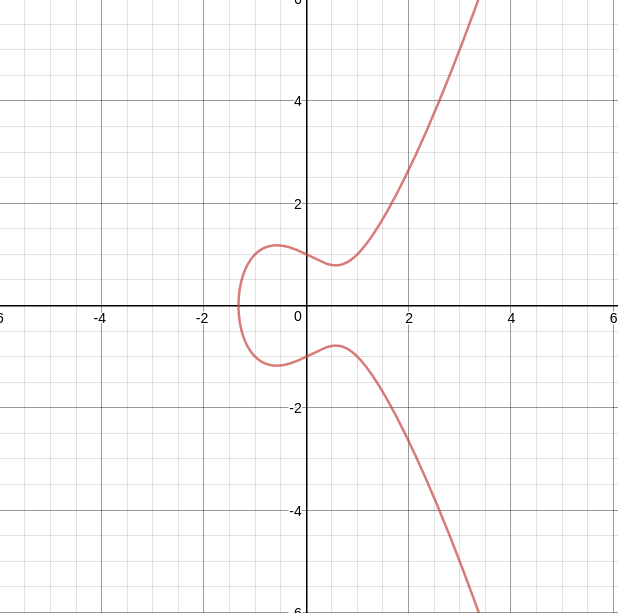
\includegraphics[width=.6\linewidth]{figures/curve1.png}
  \caption{$y^2 = x^3 -x + 1$}
  \label{fig:sub1}
\end{subfigure}%
\begin{subfigure}{.5\textwidth}
  \centering
  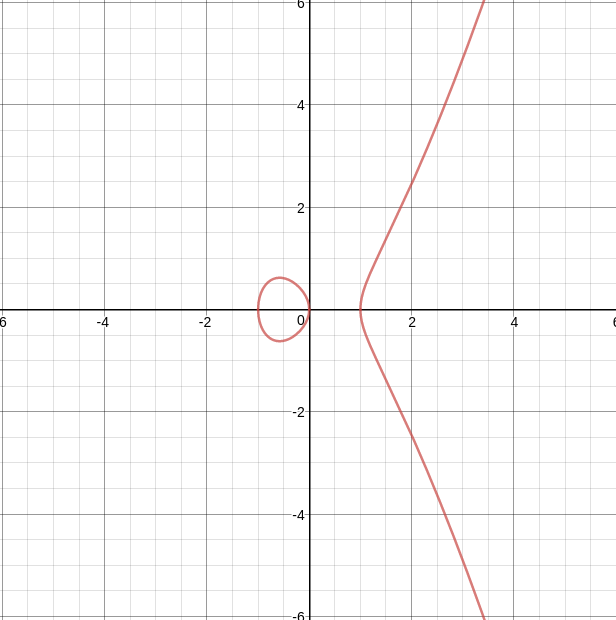
\includegraphics[width=.6\linewidth]{figures/curve2.png}
  \caption{$y^2 = x^3 - x$}
  \label{fig:sub2}
\end{subfigure}
\caption{Exemplo de duas curvas elípticas}
\label{fig:curvas}
\end{figure}

Uma outra maneira de utilizar as curvas é na criptografia de chave pública, onde a aritmética de pontos na curva é utilizada para encriptar e decriptar um dado. Sendo assim, iremos apresentar algumas curvas e suas vantagens em comparação com outros esquemas criptográficos.

Criptografia de curvas elípticas (ECC) é uma classe de algoritmos criptográficos que se baseia na aritmética de pontos de uma curva elíptica em um corpo finito $\mathbb{F}_q$ \cite{Hankerson:2003:GEC:940321}. Os algoritmos criptográficos que utilizam esse tipo de problema matemático podem se diferenciar de acordo com vários fatores, como por exemplo: o primo utilizado, a curva, corpo finito $\mathbb{F}_p$ ou $\mathbb{F}_{2^m}$, a quantidade de coordenadas utilizadas, entre outros.

A computação base de ECC é a multiplicação escalar (ECSM) descrita como: $Q = kP$. Portanto, as operações mais simples executadas em uma curva são a adição e a duplicação de pontos, sendo $R = P + Q$ e $R = 2P$ respectivamente. Dependendo da curva utilizada, essas operações são computadas de formas diferentes, podendo fazer uso de propriedades específicas da curva para obter melhor desempenho.

Seguindo a notação descrita por \cite{Hankerson:2003:GEC:940321} podemos definir uma curva elíptica $E$ como: $E: y^2 + a_1xy + a_3y = x^3 + a_2x^2 + a_4x + a_6$ sobre um corpo K. Onde $\bigtriangleup \neq 0$, essa condição garante que não existirá ponto onde a curva possui duas ou mais linhas de tangente diferentes. A linha da tangente é utilizada na operação de duplicação de um ponto. Sendo que, $\bigtriangleup$ é definido como:

\begin{align*}
\bigtriangleup &= -d_2^2d_8 - 8d_4^3 - 27d_6^2 + 9d_2d_4d_6 \\
d_2 &= a_1^2 + 4a_2 \\
d_4 &= 2a_4 + a_1a_3 \\ 
d_6 &= a_3^2 + 4a_6 \\
d_8 &= a_1^2a_6 + 4a_2a_6 - a_1a_3a_4 + a_2a_3^2 - a_4^2
\end{align*}

A curva descrita anteriormente é chamada de equação de Weiertrass, onde a mesma possui uma forma simplificada: $y^2 = x^3 + ax + b$. Essa equação é utilizada como ponto inicial para descrição de várias curvas, sendo que pode-se variar os valores de $a$ e $b$ para obter diferentes curvas. Durante a escolha de qual utilizar é possível verificar a facilidade de implementação, possibilidade de paralelização, e também o desempenho da mesma. 

O desempenho está ligado as operações executadas, como por exemplo o método Montgomery-Ladder utilizado durante a multiplicação escalar, e pelas instruções do processador que facilitam a aritmética. Na seção a seguir iremos exibir as curvas com mais ocorrência na literatura, e algumas propriedades de cada uma.

\subsection{Curvas NIST e curvas modernas}
Primeiramente iremos apresentar as curvas NIST, essas curvas são recomendações de utilização feitas pelo NIST (National Institute of Standards and Technlogy), situado nos Estados Unidos da América. As mesmas foram geradas de forma pseudo-aleatória pela NSA, e possuem ao todo são 10 corpos finitos sendo 5 corpos primos ($\mathbb{F}_p$) e 5 corpos binários ($\mathbb{F}_{2^m}$) \cite{Brown2001}.

Os corpos foram recomendados com o foco no desempenho das curvas, facilitando a aritmética utilizada. Todavia existe uma resistência da comunidade em adotar o que foi proposto, pela incerteza na existência de vulnerabilidades, inseridas para obter informações secretas pelo governo norte americano. Os corpos finitos recomendados podem ser observados a seguir, sendo P os corpos primos e B as corpos binários:

\begin{multicols}{2}
\begin{itemize}
\item P-192 \\ $\mathbb{F}_{192}$ $p = 2^{192} - 2^{64} - 1$; 
\item P-224 \\ $\mathbb{F}_{224}$ $p = 2^{224} - 2^{96} + 1$;
\item P-256 \\ $\mathbb{F}_{256}$ $p = 2^{256} - 2^{224} + 2^{192} + 2^{96} - 1$;
\item P-384 \\ $\mathbb{F}_{384}$ $p = 2^{384} - 2^{128} - 2^{96} + 2^{32} - 1$;
\item P-521 \\ $\mathbb{F}_{521}$ $p = 2^{521} - 1$;
\item B-163 \\ $\mathbb{F}_{2^{163}}$ $f(x) = x^{163} + x^7 + x^6 + x^3 + 1$;
\item B-233 \\ $\mathbb{F}_{2^{233}}$ $f(x) = x^{233} + x^{74} + 1$;
\item B-283 \\ $\mathbb{F}_{2^{283}}$ $f(x) = x^{283} + x^{12} + x^7 + x^5 + 1$;
\item B-409 \\ $\mathbb{F}_{2^{409}}$ $f(x) = x^{409} + x ^{87} + 1$;
\item B-571 \\ $\mathbb{F}_{2^{571}}$ $f(x) = x^{571} + x^{10} + x^5 + x^2 + 1$.
\end{itemize}
\end{multicols}

Nesses corpos finitos primos é recomendado utilizar as curvas pseudo-aleatórias, já no caso dos corpos binários recomenda-se, além da utilização das curvas pseudo-aleatórias, o uso da curva de Koblitz. A geração de curvas pseudo-aleatórias segue três passos: primeiramente é gerada uma semente, após a partir da semente é gerada uma curva. Por fim, é verificado se a curva gerada é resistente aos ataques conhecidos, caso não seja o processo é repetido.

Existem duas curvas elípticas que estão se destacando considerando o desempenho obtido junto à técnicas de multiplicação escalar eficiente, redução modular, entre outras. Elas são a curva de Montgomery e a curva de Edwards, onde essas possuem segurança intrínsica a ataques de canal lateral como por exemplo ataque por tempo e ataque por cache. 

Isso é verdade pois as operações na curva, o número de adições e duplicações, se baseiam no tamanho dos \textit{bits} e não no valor dos \textit{bits} da chave. Além disso, cada ECSM requisita uma adição e uma duplicação, tornando frequente o número de operações executadas a cada iteração \cite{Okeya2000}.

A curva de Montgomery tem a seguinte equação: $E: y^2 = x^3 + Ax^2 + x$. O valor do parâmetro $A$ pode ser alterado para melhorar o desempenho das multiplicações escalares. O primo mais utilizado com essa curva é o $25519$ $(2^{255}-19)$ e o valor de $A = 486662$, dessa maneira a curva é definida sobre o corpo $\mathbb{F}_{2^{255}-19}$ \cite{Dull:2015:HCM:2834659.2834708}. Essa combinação proporciona a multiplicação escalar de forma eficiente com a função Montgomery-ladder.

Uma outra curva a ser observada é a curva de Edwards. A mesma apresenta a característica de suas implementações serem regulares, o que proporciona execução segura do algoritmo. É encontrada na literatura a utilização dessa curva na forma \textit{twisted}, pelo desempenho encontrado pela combinação com o primo de Mersenne, $p = 2^{127} - 1$, e o 25519 em \cite{longa:2015, Bernstein2012} respectivamente. A equação dessa curva é a seguinte: $-x^2 + y^2 = 1 + dx^2y^2$, onde $d$ é um não quadrado em $\mathbb{F}_p^2$.

Nessa curva a soma de dois pontos segue a \textit{Edwards addition law}:
$$ (x_1,y_1) + (x_2,y_2) = (\frac{x_1y_2 + x_2y_1}{1 + xd_1x_2y_1y_2},\frac{y_1y_2 + x_1x_2}{1 - dx_1x_2y_1y_2}) $$
Já a duplicação de um ponto segue a mesma fórmula da adição, portanto a diferença é que ambos os pontos possuem os mesmos valores, sendo: $(x_1, y_1) + (x_1, y_1)$.

\subsection{Algoritmos para multiplicação escalar (ECSM) básicos}
Considerando que a principal operação em curvas elípticas é a multiplicação escalar é necessário explorar as diferentes formas de implementar esse calculo. Nessa seção serão apresentados os mais simples, resistentes ou não a ataques de canal lateral, e pequenas variações criando novos algoritmos com propriedades diferentes.

O primeiro é o método \textit{Double-and-add} (também conhecido como \textit{Double-and-add-not-always}), o mesmo é utilizado para calcular $kP$. Ele possui quatro variáveis, sendo $N$ para armazenar o resultado da operação de duplicação do ponto durante a execução, $Q$ armazena o resultado das operações, $P$ é o ponto escolhido na curva para a multiplicação escalar, e por fim $k$ é a chave utilizada na multiplicação.

É importante citar que $m$ é o tamanho da chave em bits, sendo que cada \textit{bit} da chave será utilizado nesse método, totalizando 256 execuções para uma chave de 32 \textit{bytes}. O algoritmo 1 é chamado também de \textit{left-to-right} considerando a orientação onde são percorridos os \textit{bits} da chave privada. É necessário citar que esse algoritmo não é resistente a ataques de canal lateral, sendo que existe uma variação de tempo dependendo do valor dos bits da chave.

\floatname{algorithm}{Algoritmo}
\begin{algorithm}[H]
\caption{Double-and-add left-to-right}
\begin{algorithmic} 
    \REQUIRE $P, k=(k_{d-1},\ldots,k_1,k_0)_2 \in \mathbb{N}$
    \ENSURE $Q = kP$
    \STATE $N \leftarrow P$
    \STATE $Q \leftarrow 0$
    \FOR{$i$ from $d-1$ \textbf{downto} $0$} 
        \STATE $N \leftarrow 2N$
        \IF{$k_i = 1$}
            \STATE $Q \leftarrow Q+N$
        \ENDIF
    \ENDFOR
    \RETURN Q
    \end{algorithmic}
\end{algorithm}

Uma outra maneira de percorrer os \textit{bits} de \textit{d} é do \textit{bit} menos significativo para o  mais significativo, e é conhecida como \textit{right-to-left}. A mesma apresenta pequenas diferenças em relação ao algoritmo 1 em termos do código, modificando apenas a ordem dos \textit{bits} percorridos e a ordem as operações de adição e duplicação. Já em relação à segurança esse também não é resistente a ataques de canal lateral.

\floatname{algorithm}{Algoritmo}
\begin{algorithm}[H]
\caption{Double-and-add right-to-left}
\begin{algorithmic} 
    \REQUIRE $P, k=(k_{d-1},\ldots,k_1,k_0)_2 \in \mathbb{N}$
    \ENSURE $Q = kP$
    \STATE $N \leftarrow P$
    \STATE $Q \leftarrow 0$
    \FOR{$i$ from $0$ \TO $d$} 
        \IF{$k_i = 1$}
            \STATE $Q \leftarrow Q + N$
        \ENDIF
        \STATE $N \leftarrow 2N$
    \ENDFOR
    \RETURN Q
    \end{algorithmic}
\end{algorithm}

Na seção 3.4 iremos tratar outros método de multiplicação escalar que são resistentes a ataques de canal lateral, tornando constante o número de operações executadas em cada iteração e o tempo de execução independente do valor da chave.

\subsection{Uso de tabelas precomputadas para melhorar desempenho; algoritmos de janela fixa}
Considerando a utilização de um ponto $P$ fixo, é possível executar o pré-processamento da exponenciação de $P$ e armazenar em uma tabela para ser utilizada em várias multiplicações escalares diferentes. Consequentemente existe um ganho de desempenho em relação a mesma implementação sem a utilização da tabela, pois torna rápida a multiplicação escalar onde a fatoração de $P$ é utilizada. Isso é possível considerando que o maior custo do algoritmo é na geração da tabela, tornando eficiente a partir da primeira multiplicação escalar \cite{Hankerson:2003:GEC:940321}.

Um exemplo disso é um ponto $P$ fixo, os seguintes valores são pré-computados: $2P, 2^2P, 2^3P,..., 2^mP$, sendo $m$ a quantidade de bits do multiplicador escalar $k$ \cite{Hankerson:2003:GEC:940321}. Dessa maneira qualquer operação de duplicação do ponto já foi calculada. Agora iremos apresentar um algoritmo que faz esse pré-processamento que foi proposto por Brickell, Gordon, McCurley, e Wilson. O mesmo recebeu o nome de \textit{Fixed-base windowing method for point multiplication}, e pode ser observado no algoritmo 3.

\renewcommand{\algorithmicforall}{\textbf{for each}}

\floatname{algorithm}{Algoritmo}
\begin{algorithm}[H]
\caption{Fixed-base windowing method for point multiplication}
\begin{algorithmic} 
    \REQUIRE $P, k=(k_{d-1},\ldots,k_1,k_0)_2 \in \mathbb{N}$
    \ENSURE $Q = kP$
    \STATE Compute $P_i = 2^{wi}P, 0 \le i \le d-1$
    \STATE $A \leftarrow \infty$
    \STATE $B \leftarrow \infty$
    \FOR{$j$ from $2^w-1$ \textbf{downto} $1$} 
        \FOR{\textbf{each} $i$ for $K_i = j$}
            \STATE $B \leftarrow B + P_i$
            \STATE $A \leftarrow A + B$
        \ENDFOR
    \ENDFOR
    \RETURN A
    \end{algorithmic}
\end{algorithm}


\subsection{Algoritmos regulares; atomicidade; montgomery ladder}
Para que algoritmos de multiplicação escalar sejam resistentes à ataques de canal lateral é necessário que o fluxo de execução seja regular, isso significa que as operações a serem executadas não serão alteradas de acordo com o valor da chave privada. É possível observar que com essas alterações o tempo de execução será constante, já se tornando resistência minimamente ao ataque de canal lateral de tempo.

Primeiramente iremos apresentar o algoritmo chamado \textit{Double-and-add-always}, proposto por Coron, onde o mesmo executa a adição e duplicação do ponto em todas a iterações. O pseudo-código pode ser observado no algoirtmo 4. Da mesma maneira dos outros algoritmos de multiplicação escalar apresentados os parâmetros de entrada são o ponto $P$ e o escalar $k$, e a saída é o resultado da computação $Q$.

\begin{algorithm}[H]
\caption{Double-and-add-always}
\begin{algorithmic} 
    \REQUIRE $P, k=(k_{d-1},\ldots,k_1,k_0)_2 \in \mathbb{N}$
    \ENSURE $Q = kP$
    \STATE $R_0 \leftarrow P$
    \FOR{$i$ from $d-2$ \textbf{downto} $0$} 
        \STATE $R_0 \leftarrow 2R_0$
        \STATE $R_1 \leftarrow R_0 + P$
        \STATE $b \leftarrow k_{i}$
        \STATE $R_0 \leftarrow R_b$
    \ENDFOR
    \RETURN $R_0$
    \end{algorithmic}
\end{algorithm}

Uma implementação mais promissora que a apresentada anteriormente é chamada de \textit{Atomic Double-and-Add}. Na mesma não é possível diferenciar qual operação no ponto está sendo executada. Além disso, no algoritmo o ponto principal da segurança está na execução da operação de $\oplus$ entre $b$ e os \textit{bits} da chave, sendo que a operação de $\oplus$ não vaza informações sobre a chave. O pseudocódigo do algoritmo pode ser observado no algoritmo 5, tendo entradas o ponto $P$ e o escalar $k$.

\begin{algorithm}[H]
\caption{Atomic Double-and-Add}
\begin{algorithmic} 
    \REQUIRE $P, k=(k_{d-1},\ldots,k_1,k_0)_2 \in \mathbb{N}$
    \ENSURE $Q = kP$
    \STATE $R_0 \leftarrow P$
    \STATE $R_1 \leftarrow P$
    \STATE $j \leftarrow l - 2$
    \STATE $b \leftarrow 0$
    \WHILE{$j \ge 0$} 
        \STATE $R_0 \leftarrow R_0 + R_b$
        \STATE $b \leftarrow b \oplus k_j$
        \STATE $j \leftarrow j + k_j -1$
    \ENDWHILE
    \RETURN $R_0$
    \end{algorithmic}
\end{algorithm}


Um outro algoritmo que iremos apresentar é chamado de \textit{Montgomery Ladder}, o mesmo apresenta eficiência na multiplicar escalar em comparação com os outros e possui vantagens dependendo da curva e do primo utilizado no esquema criptográfico. Primeiramente iremos exibir uma implementação genérica do algoritmo que pode ser aplicada a qualquer curva, onde ela pode ser observada no algoritmo 6.

\begin{algorithm}[H]
\caption{Montgomery-ladder}
\begin{algorithmic} 
    \REQUIRE $P, k=(k_{d-1},\ldots,k_1,k_0)_2 \in \mathbb{N}$
    \ENSURE $Q = kP$
    \STATE $R_0 \leftarrow P$
    \STATE $R_1 \leftarrow 2P$
    \FOR{$j \leftarrow l - 2$ \TO $0$} 
        \STATE $b \leftarrow k_j$
        \STATE $R_{1-b} \leftarrow R_0 + R_1$
        \STATE $R_b \leftarrow 2R_b$
    \ENDFOR
    \RETURN $R_0$
    \end{algorithmic}
\end{algorithm}

O método \textit{Montgomery-ladder} possui uma implementação mais eficientes para a curva de Montgomery com o primo 25519. Na mesma, esse método é dividido em degraus, sendo necessário os executar 255 vezes para concluir a computação \cite{Dull:2015:HCM:2834659.2834708}. São utilizadas duas entradas sendo $s$ o escalar com tamanho igual à 256 \textit{bits}, e $x_p$ a coordenada $x$ do ponto a ser multiplicado. A função \textit{cswap}, conhecida como \textit{conditional swap}, faz a troca dos valores dos dois primeiros parâmetros caso o valor de $c$ seja $1$. Essa primeira parte do algoritmo pode ser observada no algoritmo 7.

\begin{algorithm}[H]
\caption{Montgomery ladder}
\begin{algorithmic} 
    \REQUIRE $s, x_p$
    \ENSURE $X_1, Z_1$
    \STATE $X_1 \leftarrow 1$
    \STATE $Z_1 \leftarrow 0$
    \STATE $X_2 \leftarrow x_p$
    \STATE $Z_2 \leftarrow 1$
    \STATE $p \leftarrow 0$
    \FOR{$i \leftarrow 254$ \TO $0$}
        \STATE $b \leftarrow s_i$
        \STATE $c \leftarrow b \oplus p$
        \STATE $p \leftarrow b$
        \STATE $(X_1, X_2) \leftarrow cswap(X_1,X_2,c)$
        \STATE $(Z_1,Z_2) \leftarrow cswap(Z_1,Z_2,c)$
        \STATE $(X_1, Z_1, X_2, Z_2) \leftarrow ladder(x_p, X_1, Z_1, X_2, Z_2)$
    \ENDFOR
    \RETURN $(X_1,Z_1)$
    \end{algorithmic}
\end{algorithm}

No caso da operação de \textit{ladder} as operações executadas são necessárias para diminuir a quantidade de memória utilizada pelo algoritmo. Isso dificulta ataques considerando que o dado temporário não se mantém na memória. É possível observar a seguir no algoritmo 8 um pseudo-código do método de \textit{ladder}.

\begin{algorithm}[H]
\caption{Ladder}
\begin{multicols}{2}
\begin{algorithmic} 
    \REQUIRE $x_D, X_1, Z_1, X_2, Z_2$
    \ENSURE $X_1, Z_1, X_2, Z_2$
    \STATE $T_1 \leftarrow X_2 + Z_2$
    \STATE $X_2 \leftarrow X_2 - Z_2$
    \STATE $Z_2 \leftarrow X_1 + Z_1$
    \STATE $X_1 \leftarrow X_1 - Z_1$
    \STATE $T_1 \leftarrow T_1 \cdot X_1$
    \STATE $X_2 \leftarrow X_2 \cdot Z_2$
    \STATE $Z_2 \leftarrow Z_2 \cdot Z_2$
    \STATE $X_1 \leftarrow X_1 \cdot X_1$
    \STATE $T_2 \leftarrow Z_2 - X_1$
    \STATE $Z_1 \leftarrow T_2 \cdot a_24$
    
    
    \STATE $Z_1 \leftarrow Z_1 + X_1$
    \STATE $Z_1 \leftarrow T_2 \cdot Z_1$
    \STATE $X_1 \leftarrow Z_2 \cdot X_1$
    \STATE $Z_2 \leftarrow Z_2 - X_2$
    \STATE $Z_2 \leftarrow Z_2 \cdot Z_2$
    \STATE $Z_2 \leftarrow Z_2 \cdot x_D$
    \STATE $X_2 \leftarrow T_1 + X_2$
    \STATE $X_2 \leftarrow X_2 \cdot X_2$
    
    \RETURN $(X_1,Z_1)$
\end{algorithmic}
\end{multicols}
\end{algorithm}

\subsection{Protocolos de IoT que envolvem ECC}

No trabalho de \cite{SimplicioJr2016} podemos observar um protocolo de internet das coisas (IoT, do inglês Internet of Things) que utiliza criptografia de curvas elípticas. Esse protocolo é aplicado à redes de sensores sem fio que fazem o monitoramente do ambiente aplicado. Nessa rede um nó (mote) não possui grande capacidade de processamento, largura de banda, energia, memória, entre outros. Sendo assim, a comunicação entre os nós requer implementações eficientes de protocolos criptográficos, para acordo de chaves autenticada, encriptação e decriptação.

Nesse projeto foi estudado um protocolo eficiente baseado em ECC para acordo de chaves autenticadas (iSMQV, do inglês Implicitly-Certified Authenticated Key Agreement). Esse protocolo utiliza um centro gerador de chaves (KGC, do inglês Key Generation Center) para gerar o par de chaves, sendo pública e privada. Essas chaves apresentam certificado e podem ser verificadas com informações públicas. O objetivo das mesmas é a utilização para estabelecer uma chave comum entre dois nós da rede.

No protocolo iSMQV para que o nó da rede, que chamaremos de $A$, obtenha o seu par de chaves é necessário seguir os passos:
\begin{itemize}
    \item A escolhe um número aleatório $\alpha$ e computa $V = \alpha \cdot G$, sendo $G$ o gerador do grupo $\mathbb{G}$. O valor de $V$ e a sua identidade $ID_A$ são enviadas para o KGC;
    \item Então KGC verifica a identidade de $A$ e computa $V_A = V + \beta \cdot G$, para um $\beta$ aleatório;
    \item Além disso, KGC calcula o hash $h = H(ID_A, V_A)$ e cria a assinatura $s = h \cdot \beta + r$;
    \item $s$ e $V_A$ são enviados ao nó $A$;
    \item Por fim, $A$ calcula $h = H(ID_A, V_A)$, a chave privada $r_A = h \cdot \alpha + s$, e a chave pública $U_A = r_A \cdot G$.
\end{itemize}

Após cada nó ter o seu par de chaves eles podem iniciar o acordo de chaves, para então com posse de uma chave simétrica única trocar mensagens. Esse acordo é feito com o protocolo Diffie-Hellman, onde o $ID$ e $Y$ também são trocados para verificar a identidade de ambas as partes. 

Vamos apresentar o protocolo inteiro considerando dois nós que desejam se comunicar, $A$ e $B$. Cada nó escolhe um $x$ aleatório e computa $X = x \cdot G$. Esse resultado é trocado entre $A$ e $B$, e cada parte executa a multiplicação do seu $G$ pelo resultado do outro, sendo os resultados $s_A = X_B \cdot G$ e $s_B = X_A \cdot G$.

Após a troca da chave pública ela é validada e se for aprovada continuam o processo. Ambos $A$ e $B$ calculam os \textit{hashs} $d$ e $e$ da chave pública do outro e concatenam com a sua própria chave privada para computar $\sigma$. A chave secreta $K$ é computada criando um \textit{hash} de $\sigma$ e as informações públicas trocadas.

Esse é um exemplo de um protocolo com chave autenticada para acordo de chaves. É possível observar que com a utilização do protocolo Diffie-Hellman e a criptografia curvas elípticas é possível obter desempenho no acordo de chaves considerando o desempenho já apresentado nessa seção.